\documentclass[preprint,12pt]{elsarticle}

\usepackage{amssymb}

\usepackage{lineno}
\usepackage{hyperref}
\usepackage{quoting}
\usepackage{float}
\usepackage{lipsum}
\usepackage{tikz}
\usetikzlibrary{shapes,arrows,chains}
\usepackage{minted}
\usepackage{pythontex}
\usepackage{amsmath}
\usetikzlibrary{matrix,shapes,arrows,positioning,chains}

\usepackage{listings}
\usepackage{xcolor}

\definecolor{codegreen}{rgb}{0,0.6,0}
\definecolor{codegray}{rgb}{0.5,0.5,0.5}
\definecolor{codepurple}{rgb}{0.58,0,0.82}
\definecolor{backcolour}{rgb}{1,1,1}

\lstdefinestyle{mystyle}{
    backgroundcolor=\color{backcolour},   
    commentstyle=\color{codegreen},
    keywordstyle=\color{magenta},
    stringstyle=\color{codepurple},
    basicstyle=\ttfamily\footnotesize,
    breakatwhitespace=false,         
    breaklines=true,                 
    captionpos=b,                    
    keepspaces=true,                                 
    showspaces=false,                
    showstringspaces=false,
    showtabs=false,                  
    tabsize=2
}

\lstset{style=mystyle}


\newcommand{\comment}[1]{}

\begin{document}
	
	\tikzset{
		desicion/.style={
			diamond,
			draw,
			text width=3em,
			text badly centered,
			inner sep=0pt
		},
		block/.style={
			rectangle,
			draw,
			text width=15em,
			text centered,
			rounded corners
		},
		cloud/.style={
			draw,
			ellipse,
			minimum height=2em
		},
		descr/.style={
			fill=white,
			inner sep=2.5pt
		},
		connector/.style={
			-latex,
			font=\scriptsize
		},
		rectangle connector/.style={
			connector,
			to path={(\tikztostart) -- ++(#1,0pt) \tikztonodes |- (\tikztotarget) },
			pos=0.5
		},
		rectangle connector/.default=-2cm,
		straight connector/.style={
			connector,
			to path=--(\tikztotarget) \tikztonodes
		}
	}

\begin{frontmatter}

\title{Compressione di immagini tramite DCT\\
\large{Attraverso l'utilizzo di Python}
\vspace{5mm}\\ \normalsize{\texttt{https://github.com/nicoripa/MCS\_Project/}}}

\author{Lorenzo Rovida, Nicolò Ripamonti\\
	\small{ \href{mailto:l.rovida1@campus.unimib.it}{l.rovida1@campus.unimib.it},  \href{mailto:n.ripamonti@campus.unimib.it}{n.ripamonti@campus.unimib.it}\\817151, 816171}}

\address{Dipartimento di Informatica, Sistemi e Comunicazione, Universitá degli Studi di Milano-Bicocca, Milano, Italia}


\begin{abstract}
Lo scopo di questo progetto è quello di utilizzare l’implementazione dell'operazione matematica denominata \textbf{DCT2} in un ambiente \textit{open source} e di studiare gli effetti di un algoritmo di compressione di tipo jpeg (senza utilizzare una matrice di quantizzazione) sulle delle immagini in toni di grigio di formato \textit{bitmap}.
Il progetto si divide in tue macro parti:
\begin{description}
\item[Parte 1] Implementare la DCT2  in un ambiente open source a scelta e confrontare i tempi di esecuzione con la DCT2 ottenuta usando la libreria dell’ambiente utilizzato. In particolare, bisogna utilizzare array quadrati $N \times N$ con $N$ crescente e rappresentare su un grafico i tempi di esecuzione dei due algoritmi.
\item[Parte 2] Scrivere un software in grado di far scegliere all'utente un'immagine in formato bitmap e successivamente comprimere tale immagine utilizzando la DCT2, tagliare le frequenze che l'utente sceglie di eliminare, utilizzare l'inversa della DCT e far visualizzare a schermo l'immagine originale con quella ottenuta dopo aver modificato le frequenze.
\end{description}
\end{abstract}

\end{frontmatter}

\newpage

\section{Introduzione}
\subsection{Discrete Cosine Transform}
La trasformata discreta del coseno o DCT, è la più diffusa funzione che provvede alla compressione spaziale, capace di rilevare le variazioni di informazione tra un'area e quella contigua di un'immagine digitale trascurando le ripetizioni.

È una trasformata simile alla trasformata discreta di Fourier (DFT), ma fa uso solo di numeri reali.

La variante più comune della trasformata discreta del coseno è la DCT tipo II che è spesso chiamata semplicemente DCT; la sua inversa, la DCT tipo III è, in corrispondenza, chiamata spesso DCT inversa o IDCT. 

La DCT, e in particolare la DCT-II, è spesso usata nell'elaborazione dei segnali e delle immagini, specialmente per la compressione con perdita (compressione di tipo \textbf{lossy}). L'algoritmo JPEG è basato sulla Trasformata discreta del coseno bidimensionale (DCT2), che viene applicata su blocchi di 8x8 pixel, i cui risultati sono poi quantizzati e compressi con tecniche basate sull'entropia (come la Codifica di Huffman o la Codifica aritmetica).

\bigskip
La formula che descrive il funzionamento della DCT bidimensionale è la seguente:
\begin{eqnarray*}
c_{kl} = a_{kl} \sum_{i=0}^{N-1} \sum_{j=0}^{M-1} f_{ij} \,  cos\left(k\pi \frac{2i+1}{2N}\right) \, cos\left(l\pi \frac{2j+1}{2M}\right)
\end{eqnarray*}

Dove $a_{kl} = a_{k}^{N} a_{l}^{M}$:
\begin{eqnarray*}
a_{00} = \frac{1}{\sqrt{NM}},\; e \; a_{k0} = a_{0l} = \sqrt{\frac{2}{NM}},\; a_{kl} = \frac{2}{\sqrt{NM}}, \; k, l \geq 1.
\end{eqnarray*}

Mentre $f_{ij}$ sono gli indici bidimensionali:
\begin{eqnarray*}
\textbf{f} = (f_{ij}), \; i=0, ..., N-1, j=0, ..., M-1.
\end{eqnarray*}

\subsection{.Formato bitmap}
Windows bitmap è un formato dati utilizzato per la rappresentazione di immagini \textbf{raster} sui sistemi operativi Microsoft Windows. Noto soprattutto come formato di file, fu introdotto con Windows 3.0 nel 1990.
Le bitmap, come sono comunemente chiamati i file d'immagine di questo tipo, hanno generalmente l'estensione \textbf{.bmp}.

Sono state sviluppate tre versioni del formato bitmap. La prima e più comunemente utilizzata è la versione 3: non esistono versioni antecedenti. Le versioni successive 4 e 5 si incontrano piuttosto raramente.

Il formato di file Windows bitmap nella versione 3 permette operazioni di lettura e scrittura molto veloci e senza perdita di qualità, ma richiede generalmente una maggior quantità di memoria rispetto ad altri formati analoghi.

Le immagini bitmap possono avere una profondità di 1, 4, 8, 16, 24 o 32 bit per pixel. Le bitmap con 1, 4 e 8 bit contengono una tavolozza per la conversione dei (rispettivamente 2, 16 e 256) possibili indici numerici nei rispettivi colori. Nelle immagini con profondità più alta il colore non è indicizzato bensì codificato direttamente nelle sue componenti cromatiche RGB; con 16 o 32 bit per pixel alcuni bit possono rimanere inutilizzati.

Nel caso in esame le immagini in formato \textit{.bmp} sono state scelte con colori in scala di grigi, ovvero immagini con una profondità di 8 bit. Tali bit servono per convertire gli indici numerici nei rispettivi bit, in questo caso da 0, che identifica il colore nero, a 255, che identifica il colore bianco. Tutti i valori tra l'1 e il 254 sono tutte le possibili varianti di grigio.

\subsection{Calcolatore utilizzato}
Per effettuare i calcoli sugli script è stato utilizzato un MacBook Pro 2016 con le seguenti caratteristiche hardware:
\begin{description}
\item[Processore] 2 GHz Intel Core i5 dual-core
\item[Architettura] CPU x64
\item[Memoria] 8 GB 1867 MHz LPDDR3
\item[Scheda grafica] Intel Iris Graphics 540 1536 MB
\end{description}

\newpage

\section{Ambiente di sviluppo}

L'ambiente di sviluppo scelto per il progetto, sia per la parte 1 che per la parte 2, è stato \textbf{Python}.

\medskip
\begin{description}
\item[Versione:] 3.7.3
\item[Referenze:] \href{https://www.python.org}{Sito} - \href{https://docs.python.org/3/}{Documentazione}
\end{description}

\begin{figure}[H]
	\centering
	
\includegraphics[width=.3\linewidth]{logo}
\end{figure}

Python è un linguaggio di programmazione di più "alto livello" rispetto alla maggior parte degli altri linguaggi. È orientato a oggetti, ma non in maniera ferrea come ad esempio Java; adatto, tra gli altri usi, a sviluppare applicazioni distribuite, scripting, computazione numerica e system testing.

È un linguaggio multi-paradigma che ha tra i principali obiettivi: dinamicità, semplicità e flessibilità. Supporta il paradigma object oriented, la programmazione strutturata e molte caratteristiche di programmazione funzionale e riflessione.

Le caratteristiche più immediatamente riconoscibili di Python sono le variabili non tipizzate e l'uso dell'indentazione per la definizione delle specifiche. \\

\section{Librerie}
Nello specifico sono state utilizzate diverse librerie sia per l'implementazione del codice della parte 1 del progetto, sia per la parte 2.

Esse nello specifico sono:
\begin{description}
\item[TkInter] \href{https://docs.python.org/3/library/tk.html}{Sito} - Versione 3.8.3 \\
\`E una libreria che permette di creare interfacce grafiche nella programmazione con Python, molto conosciuta e utilizzata per la sua leggerezza e stabilità.

\item[SciPy] \href{https://www.scipy.org}{Sito} - Versione 1.19.0 \\
\`E una libreria open source di algoritmi e strumenti matematici. Contiene moduli per l'ottimizzazione, per l'algebra lineare, elaborazione di segnali ed immagini  e altri strumenti comuni nelle scienze e nell'ingegneria. Trova utilizzo in quei programmatori che usano anche MATLAB. All'interno di SciPy sono presenti diversi pacchetti tra cui \textbf{fftpack}, che contiene tutti gli algoritmi della trasformata discreta di Fourier e anche classi per l'implementazione della trasformata discreta del coseno (\textbf{DCT});

\item[NumPy] \href{https://numpy.org}{Sito} - Versione 1.18.4 \\
\`E un pacchetto per l'elaborazione scientifica con Python. In particolare questo pacchetto è stato utilizzato per effettuare operazioni su array bidimensionali;

\item[MatplotLib] \href{https://matplotlib.org}{Sito} - Versione 3.2.1 \\
\`E una libreria completa per la creazione di visualizzazioni statiche, animate e interattive. Nel nostro interesse è stata usata per stampare le immagini nella conclusione dello script della seconda parte del progetto;

\item[Random] \href{https://docs.python.org/3.8/library/random.html}{Sito} - Versione 3.0 \\
Questo modulo implementa generatori di numeri pseudo-casuali per varie distribuzioni. \`E stata utilizzata questa libreria per la generazione di matrici casuali per lo studio dei tempi di esecuzione delle DCT nella prima parte del progetto;

\item[Time] \href{https://docs.python.org/3/library/time.html}{Sito} - Versione 3.7 \\
Questo modulo offre varie funzioni correlate al tempo. Utilizzata per la misurazione dei tempi di esecuzione delle CDT nella prima parte del progetto;

\item[CV2] \href{https://docs.opencv.org/master/index.html}{Sito} - Versione 4.3.0 \\
\`E un modulo facente parte della libreria OpenCV. CV2 è stata utilizzata all'interno dell'interfaccia grafica per poter far scegliere all'utente il file .bmp.
\end{description}

\newpage

\section{Parte 1 - Confronto implementazioni DCT}
Come spiegato all'inizio dell'elaborato, nella prima parte del progetto il compito è quello di creare un algoritmo di compressione del tipo DCT e confrontare i tempi di esecuzione con un algoritmo DCT implementato da una libreria.

\subsection{Diagramma}
Di seguito viene presentato un diagramma a blocchi che spiega in maniera veloce come è avvenuta l'implementazione dell'intera parte 1.

\begin{center}
\begin{tikzpicture}
\matrix (m)[matrix of nodes, column  sep=3cm,row  sep=10mm, align=center, nodes={rectangle,draw, anchor=center} ]{
	|[block]| {\textbf{Start}}       \\
	|[block]| {\texttt{main()} \\ Definizione del Main dello script}     \\
	|[block]| {\texttt{img = matrice\_random(dim)} \\ Calcolo di una matrice quadrata di valori interi random di dimensione \texttt{dim}}     \\
	|[block]| {\texttt{img\_slow = dct\_manual(img)} \\ Metodo per il calcolo manuale della DCT}     \\
	|[block]| {\texttt{img\_fast = dct(img)} \\ Metodo per il calcolo tramite libreria della DCT}     \\
	|[block]| {\textbf{End}}    \\
};
\path [>=latex,->] (m-1-1) edge (m-2-1);
\path [>=latex,->] (m-2-1) edge (m-3-1);
\path [>=latex,->] (m-3-1) edge (m-4-1);
\path [>=latex,->] (m-4-1) edge (m-5-1);
\path [>=latex,->] (m-5-1) edge (m-6-1);
\end{tikzpicture}
\end{center}

\newpage

\subsection{Implementazione}

Di seguito viene spiegato approfonditamente come opera lo script.


\begin{enumerate}
\item Nella funzione {\texttt{main()} viene implementato un ciclo {\texttt{while} dove avvengono tutte le operazioni. \`E stato scelto questo metodo per poter implementare uno script che faccia in automatico tutte le operazioni su matrici quadrate di dimensione sempre maggiore, ovvero la dimensione è di $100 \cdot n$, dove $n = 1, 2,  \dots, 10$;
\begin{lstlisting}[language=Python]
dim = 100
    while (dim <= 1000):
        img = matrice_random(dim)
        
        time1 = time.time()
        dct_fftpack_2d(img)
        time2 = time.time()
        
        tempi_scipy.append(time2 - time1)
        
        time1 = time.time()
        dct_manual_2d(img)
        time2 = time.time()
        
        tempi_manual.append(time2 - time1)
        
        dimensioni.append(dim)
        
        dim += 100
\end{lstlisting}

\item Viene chiamata la funzione {\texttt{matrice\_random()} che crea un array bidimensionale di valori random compresi tra $0$ e $256$, ovvero i valori che corrispondono alla scala di grigi in formato bitmap. Questa funzione prende in ingresso il valore che corrisponde alla dimensione che si vuole dare alla matrice;
\begin{lstlisting}[language=Python]
def matrice_random(dim):
    img = np.arange(dim * dim).reshape(int(dim), int(dim))
    
    m = img.shape[0]
    
    for i in range(0, m):
        for j in range(0, m):
            img[i][j] = random.randrange(256)
            
    img[0][0] = random.randrange(256)
            
    return img
\end{lstlisting}

\item Viene calcolata la DCT della libreria ScyPy e i tempi di esecuzione;
\begin{lstlisting}[language=Python]
def dct_fftpack_2d(x):
    return dct(np.transpose(dct(np.transpose(x), type = 2, norm = 'ortho')), \
               type = 2, norm='ortho')
\end{lstlisting}

\item Viene calcolata la DCT manuale e i tempi di esecuzione. La DCT viene implementata come segue;
\begin{lstlisting}[language=Python]
def dct_manual_2d(x):
    return dct_manual(np.transpose(dct_manual(np.transpose(x))))
    
def dct_manual(x):
    N = len(x)

    print(type(x[0]))
    c = []
    
    for k in range(0, N):
        somma = 0
        for i in range(0, N):
            somma = somma + (x[i] * math.cos(math.pi * k * (2 * i + 1) / (2 * N)))
    
        if k == 0:
            alpha = math.sqrt(1 / N)
        else:
            alpha = math.sqrt(2 / N)
            
        c.append(somma * alpha)
            
    return c
\end{lstlisting}

\item Vengono stampati in console tutti i tempi di esecuzione delle due DCT per ogni dimensione dell'array bidimensionale;
\begin{lstlisting}[language=Python]
 plot(dimensioni, tempi_manual, tempi_scipy)
    print('Tempi Scipy: ')
    print(tempi_scipy)
    print('Tempi manual: ')
    print(tempi_manual)
\end{lstlisting}


\end{enumerate}


\subsection{Risultati}
I risultati della prima parte del progetto riguardano il confronto dei tempi d'esecuzione della DCT2. In particolare il confronto è stato fatto tra una DCT implementata a mano e la funzione DCT del pacchetto SciPy.fftpack.

Gli array bidimensionali utilizzati di dimensione $N \times N$ sono stati creati in maniera casuale e sono state scelte dimensioni che variano da $100 \times 100$ a $1000 \times 1000$. Non sono state scelte dimensioni maggiori, sia per motivi di eccessivo tempo di calcolo, sia perché un'array $1000 \times 1000$ rispecchia un'immagine di $1000 \times 1000$ pixel, definizione già abbastanza alta, paragonabile in termini di numero di pixel al formato HD a 720p.

Durante l'implementazione abbiamo fatto molta attenzione che il nostro algoritmo venisse implementato correttamente confrontando sempre i risultati degli array dopo il calcolo di entrambe le DCT.

\begin{figure}[H]
	\centering
	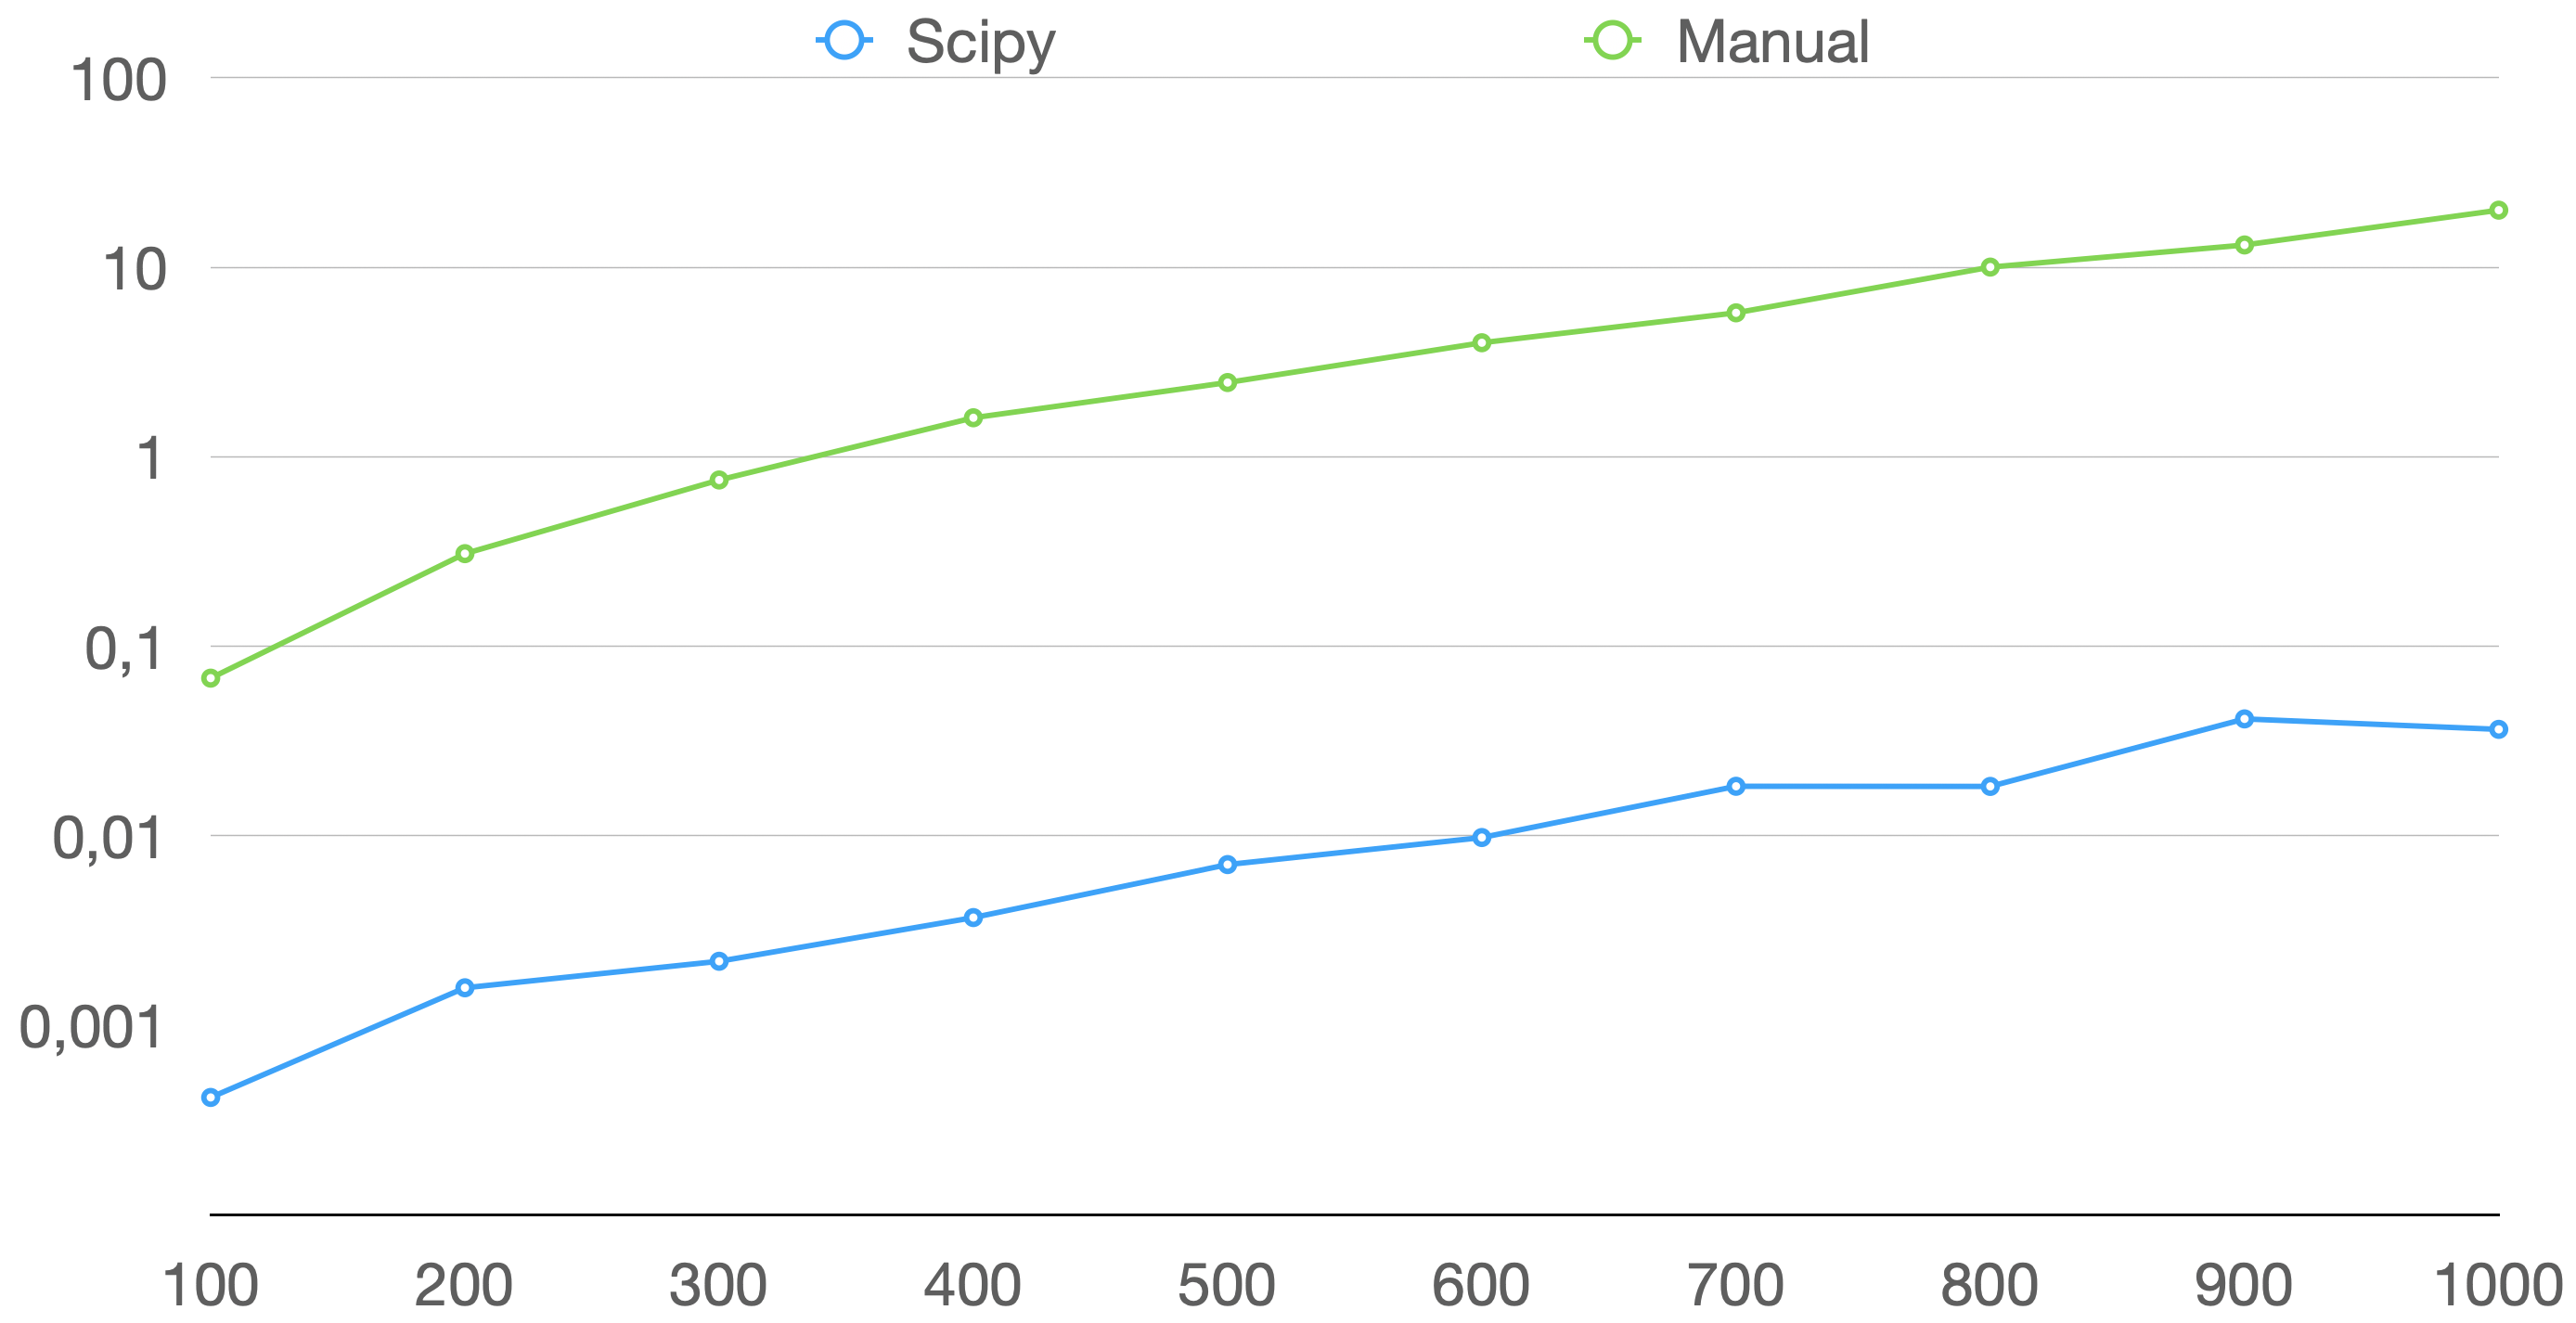
\includegraphics[width=\linewidth]{grafico}
\end{figure}

Nella figura sopra si possono notare come i tempi della DCT implementata a mano (Manual) siano nettamente superiori rispetto alla DCT implementata dal pacchetto di Python. Questo è del tutto normale in quanto le librerie sono sicuramente implementate meglio e più efficienti.

\newpage
Nella figura sotto sono riportati in una tabella tutti i tempi di esecuzione della DCT.

\begin{figure}[H]
	\centering
	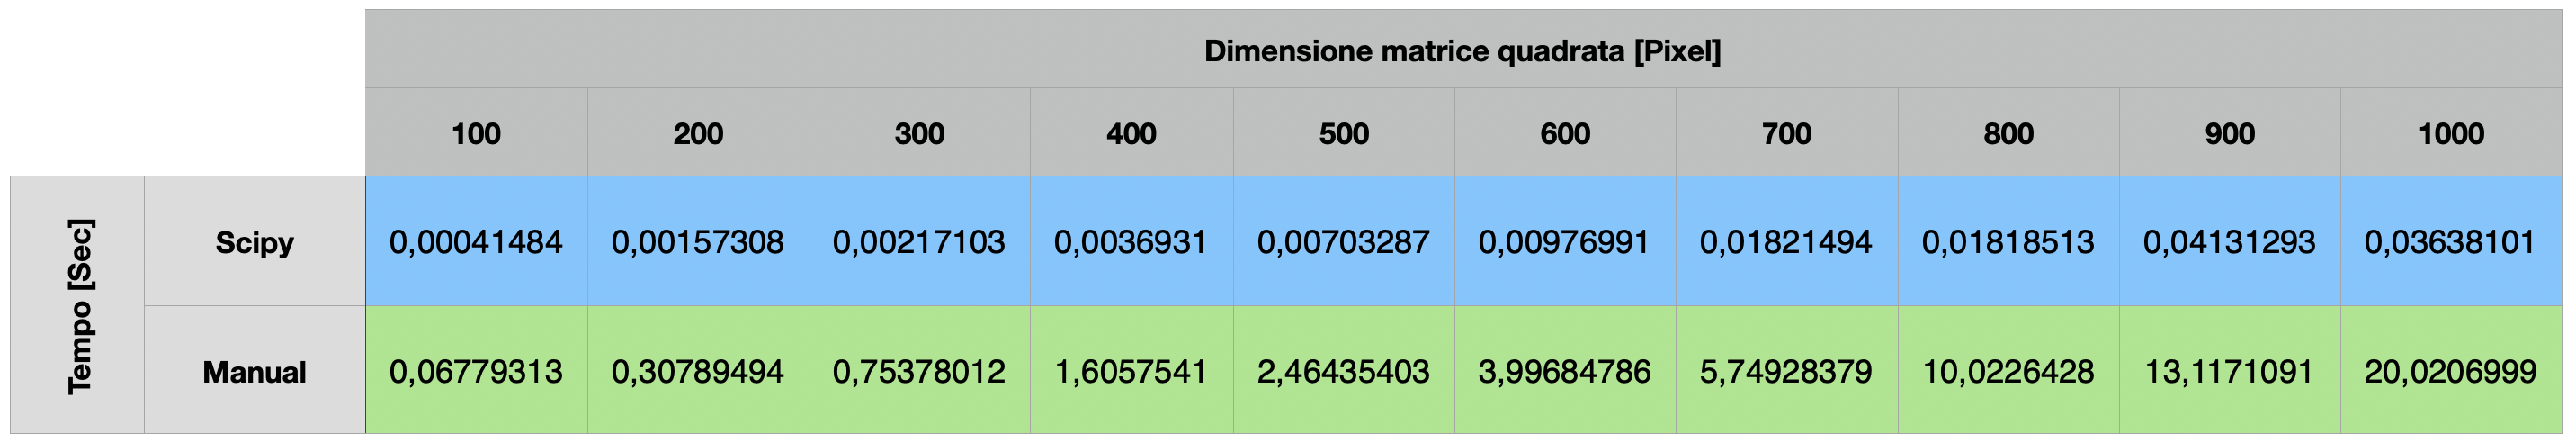
\includegraphics[width=\linewidth]{tabella}
\end{figure}

Si ricorda che i tempi di un algoritmo per DCT2 implementato da una libreria sono di circa $O(N^2 logN)$, mentre i tempi di esecuzione di una DCT2 manuale si aggirano intorno a $O(N^3)$, dove con $N$ si intende ovviamente la dimensione della matrice.

Detto ciò, i risultati finali dei tempi rispecchiamo a pieno tale regola, quindi possiamo tenerci soddisfatti circa la prima parte del progetto. 

\newpage

\section{Parte 2 - Interfaccia grafica per la compressione di immagini}
Come spiegato all'inizio dell'elaborato, la seconda parte del progetto si occupa di implementare un interfaccia grafica che permetta all'utente di effettuare una compressione da .bmp a .jpg

Nel dettaglio il programma implementato elabora l'immagine .bmp come segue.

I valori $F$ e $d$ scelti dall'utente servono per l'elaborazione e la compressione dell'immagine nel seguente modo:
\begin{description}
\item[F] è un intero che verrà utilizzato per la divisione in blocchi dell'immagine. Tali blocchi avranno dimensione $F \times F$ ed è proprio su di essi che verrà calcolata la DCT.
\item[d] è il valore intero che serve per eliminare le frequenze all'interno dei blocchi una volta calcolata la DCT. Tale valore deve essere un numero intero compreso tra $0$ e $2F-2$, perché le frequenze vengono eliminate sui blocchi $F \times F$, dove il valore che ha indici $k$ ed $l$ del blocco viene eliminato se $k + l \geq d$. 
\begin{figure}[H]
	\centering
	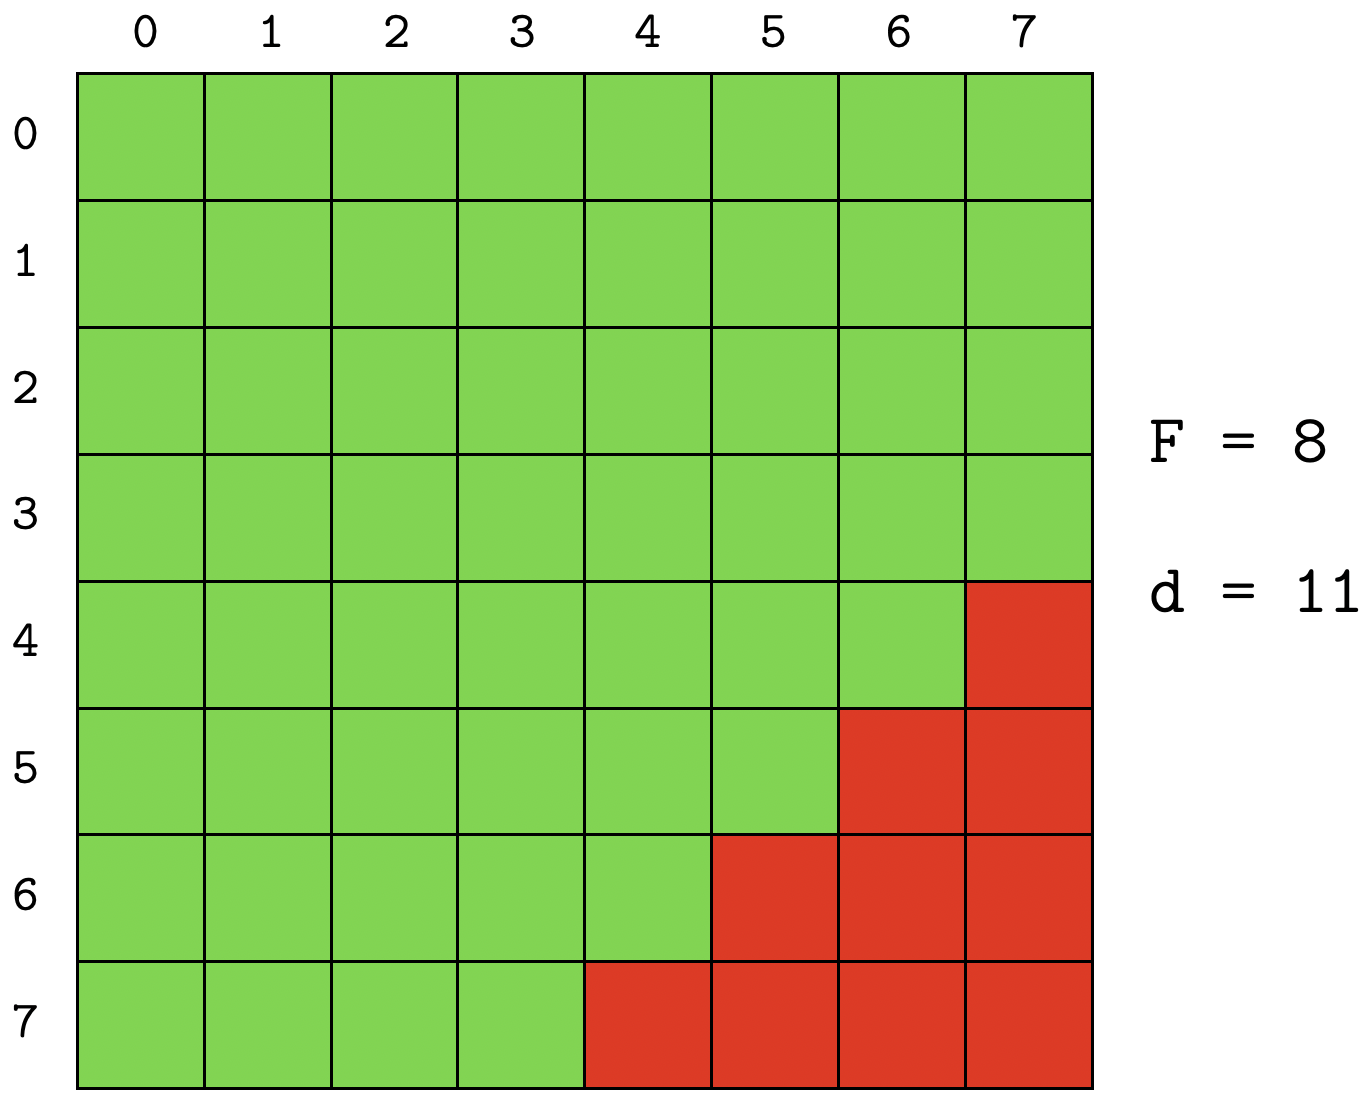
\includegraphics[width=0.5\linewidth]{esempio}
\end{figure}
\end{description}

\subsection{Diagramma}

\vspace{3mm}

\begin{tikzpicture}
\matrix (m)[matrix of nodes, column  sep=2cm,row  sep=8mm, align=center, nodes={rectangle,draw, anchor=center} ]{
	|[block]| {\textbf{Start}} \\
	|[block]| {\texttt{main()} \\ Definizione del Main in cui viene implementata l'interfaccia per scegliere dal Filesystem un'immagine in formato \texttt{.bmp}}               &          |[block]| {\texttt{lista\_blocchi\_inversa = applica\_dct(lista\_blocchi, d, f)} \\ Metodo in cui viene implementato il calcolo della DCT2, il taglio delle frequenze $c_{kl}$ con $k + l \geq d$}                                  \\
	|[block]| {\texttt{open\_file()} \\ Metodo utilizzato per l'apertura del file \texttt{.bmp}}          &       |[block]| {\texttt{img\_compressa = ricomponi(img, lista\_blocchi\_inversa, f)} \\ Metodo in cui vengono ricomposti nell'ordine giusto tutti i blocchi compressi con la DCT2}                                      \\
	|[block]| {\texttt{main\_function(F, d)} \\ Funzione principale per l'implementazione del software, F e d sono i parametri scelti dall'utente all'interno della funzione \texttt{main()}}    &    |[block]| {\texttt{plot(img, img\_compressa)} \\ Metodo per il disegno dell'immagine originale, affiancata a quella compressa con la DCT2}                                         \\
	|[block]| {\texttt{lista\_blocchi = suddividi(img, F)} \\ Metodo per suddividere l’immagine in blocchi quadrati di dimensioni $F \times F$ partendo in alto a sinistra, scartando gli avanzi}         &           |[block]| {\textbf{Stop}}                                   \\
	|[block]| {\texttt{lista\_blocchi\_inversa = applica\_dct(lista\_blocchi, d, f)} \\ Metodo in cui viene implementato il calcolo della DCT2, il taglio delle frequenze $c_{kl}$ con $k + l \geq d$}                               \\
};
\path [>=latex,->] (m-1-1) edge (m-2-1);
\path [>=latex,->] (m-2-1) edge (m-3-1);
\path [>=latex,->] (m-3-1) edge (m-4-1);
\path [>=latex,->] (m-4-1) edge (m-5-1);
\path [>=latex,->] (m-5-1) edge (m-6-1);

\path [>=latex,->] (m-2-2) edge (m-3-2);
\path [>=latex,->] (m-3-2) edge (m-4-2);
\path [>=latex,->] (m-4-2) edge (m-5-2);



\end{tikzpicture}

\subsection{Implementazione}
Di seguito viene spiegato approfonditamente come opera il programma.
\begin{enumerate}
\item Crea una lista di blocchi $F \times F$ dell'immagine importata partendo dall'alto a sinistra, eliminando li scarti sotto e a destra qualora ce ne siano;

\begin{lstlisting}[language=Python]
while (i + f < img.shape[0]):
        while(j + f < img.shape[1]):
            blocco = img[i:i+f,j:j+f]
            lista_blocchi.append(blocco)
            j = j + f
        i = i + f
        j = 0
\end{lstlisting}

\item Viene applicata la DCT ad ogni blocco;
\begin{lstlisting}[language=Python]
 for f in lista_blocchi:
        c = dct(np.transpose(dct
        		(np.transpose(f), norm='ortho')), norm='ortho')
\end{lstlisting}

\item Vengono eliminate le frequente utilizzando come valore $d$;
\begin{lstlisting}[language=Python]
for k in range(0, c.shape[0]):
            for l in range(0, c.shape[1]):
                if k + l >= d:
                    c[k, l] = 0
\end{lstlisting}

\item Viene applicata la DCT inversa ad ogni blocco;
\begin{lstlisting}[language=Python]
ff = idct(np.transpose(idct
				(np.transpose(c), norm='ortho')), norm='ortho')
\end{lstlisting}

\item Vengono arrotondati i valori di ogni blocco all'intero più vicino e, i valori minori di $0$ vengono resi uguali a $0$, mentre i valori maggiori di $255$ vengono resi uguali a $255$;
\begin{lstlisting}[language=Python]
for i in range(0, ff.shape[0]):
            for j in range(0, ff.shape[1]):
                ff[i,j] = int(ff[i,j])

                if ff[i, j] < 0:
                    ff[i,j] = 0
                    
                elif ff[i,j] > 255:
                    ff[i,j] = 255
\end{lstlisting}

\item Viene ricomposta l'immagine;
\begin{lstlisting}[language=Python]
    i = 0
    j = 0
    index = 1
    while (i + f < img.shape[0]):
        while(j + f  < img.shape[1]):
            j = j + f
            if j + f < img.shape[1]:
                col = np.hstack((col, lista_blocchi_inversa[index]))
                index = index + 1

        i = i + f
        j = 0
        colonne.append(col)
        if index < len(lista_blocchi_inversa):
            col = lista_blocchi_inversa[index]
        index = index + 1

    img_compressa = colonne[0]

    for i in range(1, len(colonne)):
        img_compressa = np.vstack((img_compressa, colonne[i]))
\end{lstlisting}

\item Viene visualizzata a schermo l'immagine originale affiancata dall'immagine ottenuta dopo aver eliminato le frequenze.
\begin{lstlisting}[language=Python]    
    fig = Figure(figsize=(5, 4), dpi=100)
    t = np.arange(0, 3, .01)
    fig.add_subplot(121).imshow(img)
    fig.add_subplot(122).imshow(img_compressa)
\end{lstlisting}

\end{enumerate}

\newpage

\subsection{Risultati}
Il software creato permette di utilizzare la formula della DCT su immagini in formato bitmap in scala di grigi.
Tale programma di presenta con una semplice interfaccia grafica che facilita l'utente nelle scelta dell'immagine .bmp da scegliere tra i propri file.

\begin{figure}[H]
	\centering
	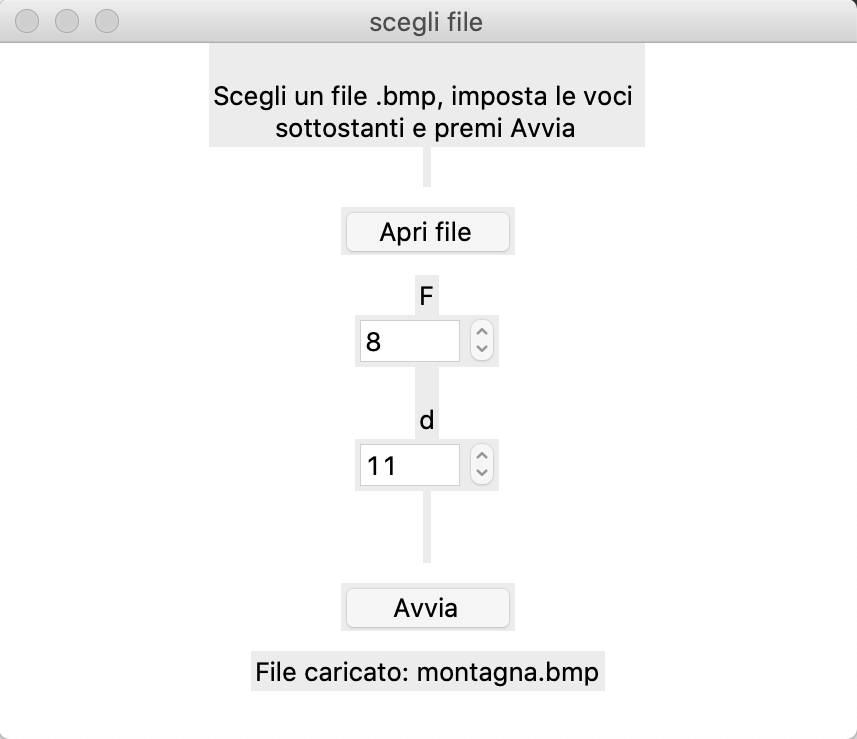
\includegraphics[width=0.5\linewidth]{gui}
\end{figure}

Una volta caricato il file e scelti i valori $F$ e $d$, l'utente può premere il tasto \textit{Avvia} e aspettare che il programma elabori il risultato, per poi farlo visualizzare all'utente.

Se $d$ non è compreso tra $0$ e $2F-2$, il programma mostra un messaggio di errore e termina l'esecuzione.
\begin{figure}[H]
	\centering
	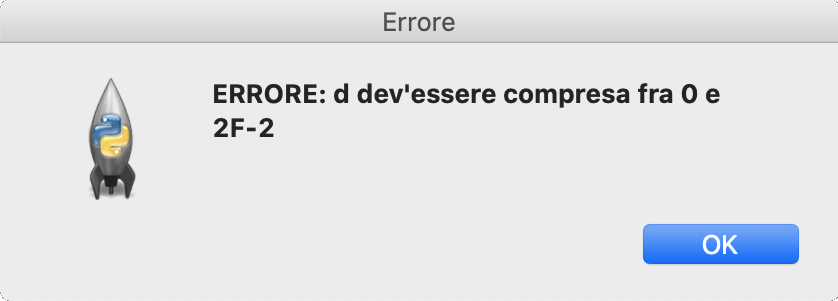
\includegraphics[width=0.55\linewidth]{errore}
\end{figure}

Verrà visualizzato un errore anche nel caso l'utente scelga un valore di \textit{F} maggiore di almeno una delle due dimensioni dell'immagine (righe e/o colonne).

Se i dati inseriti sono consistenti e l'immagine viene letta correttamente, il risultato sarà stampato su una schermata apposita in cui verrà visualizzata anche l'immagine originale.
Le due immagini (originale a sinistra, compressa a destra) saranno quindi confrontabili a "occhio".



\begin{figure}[H]
	\centering
	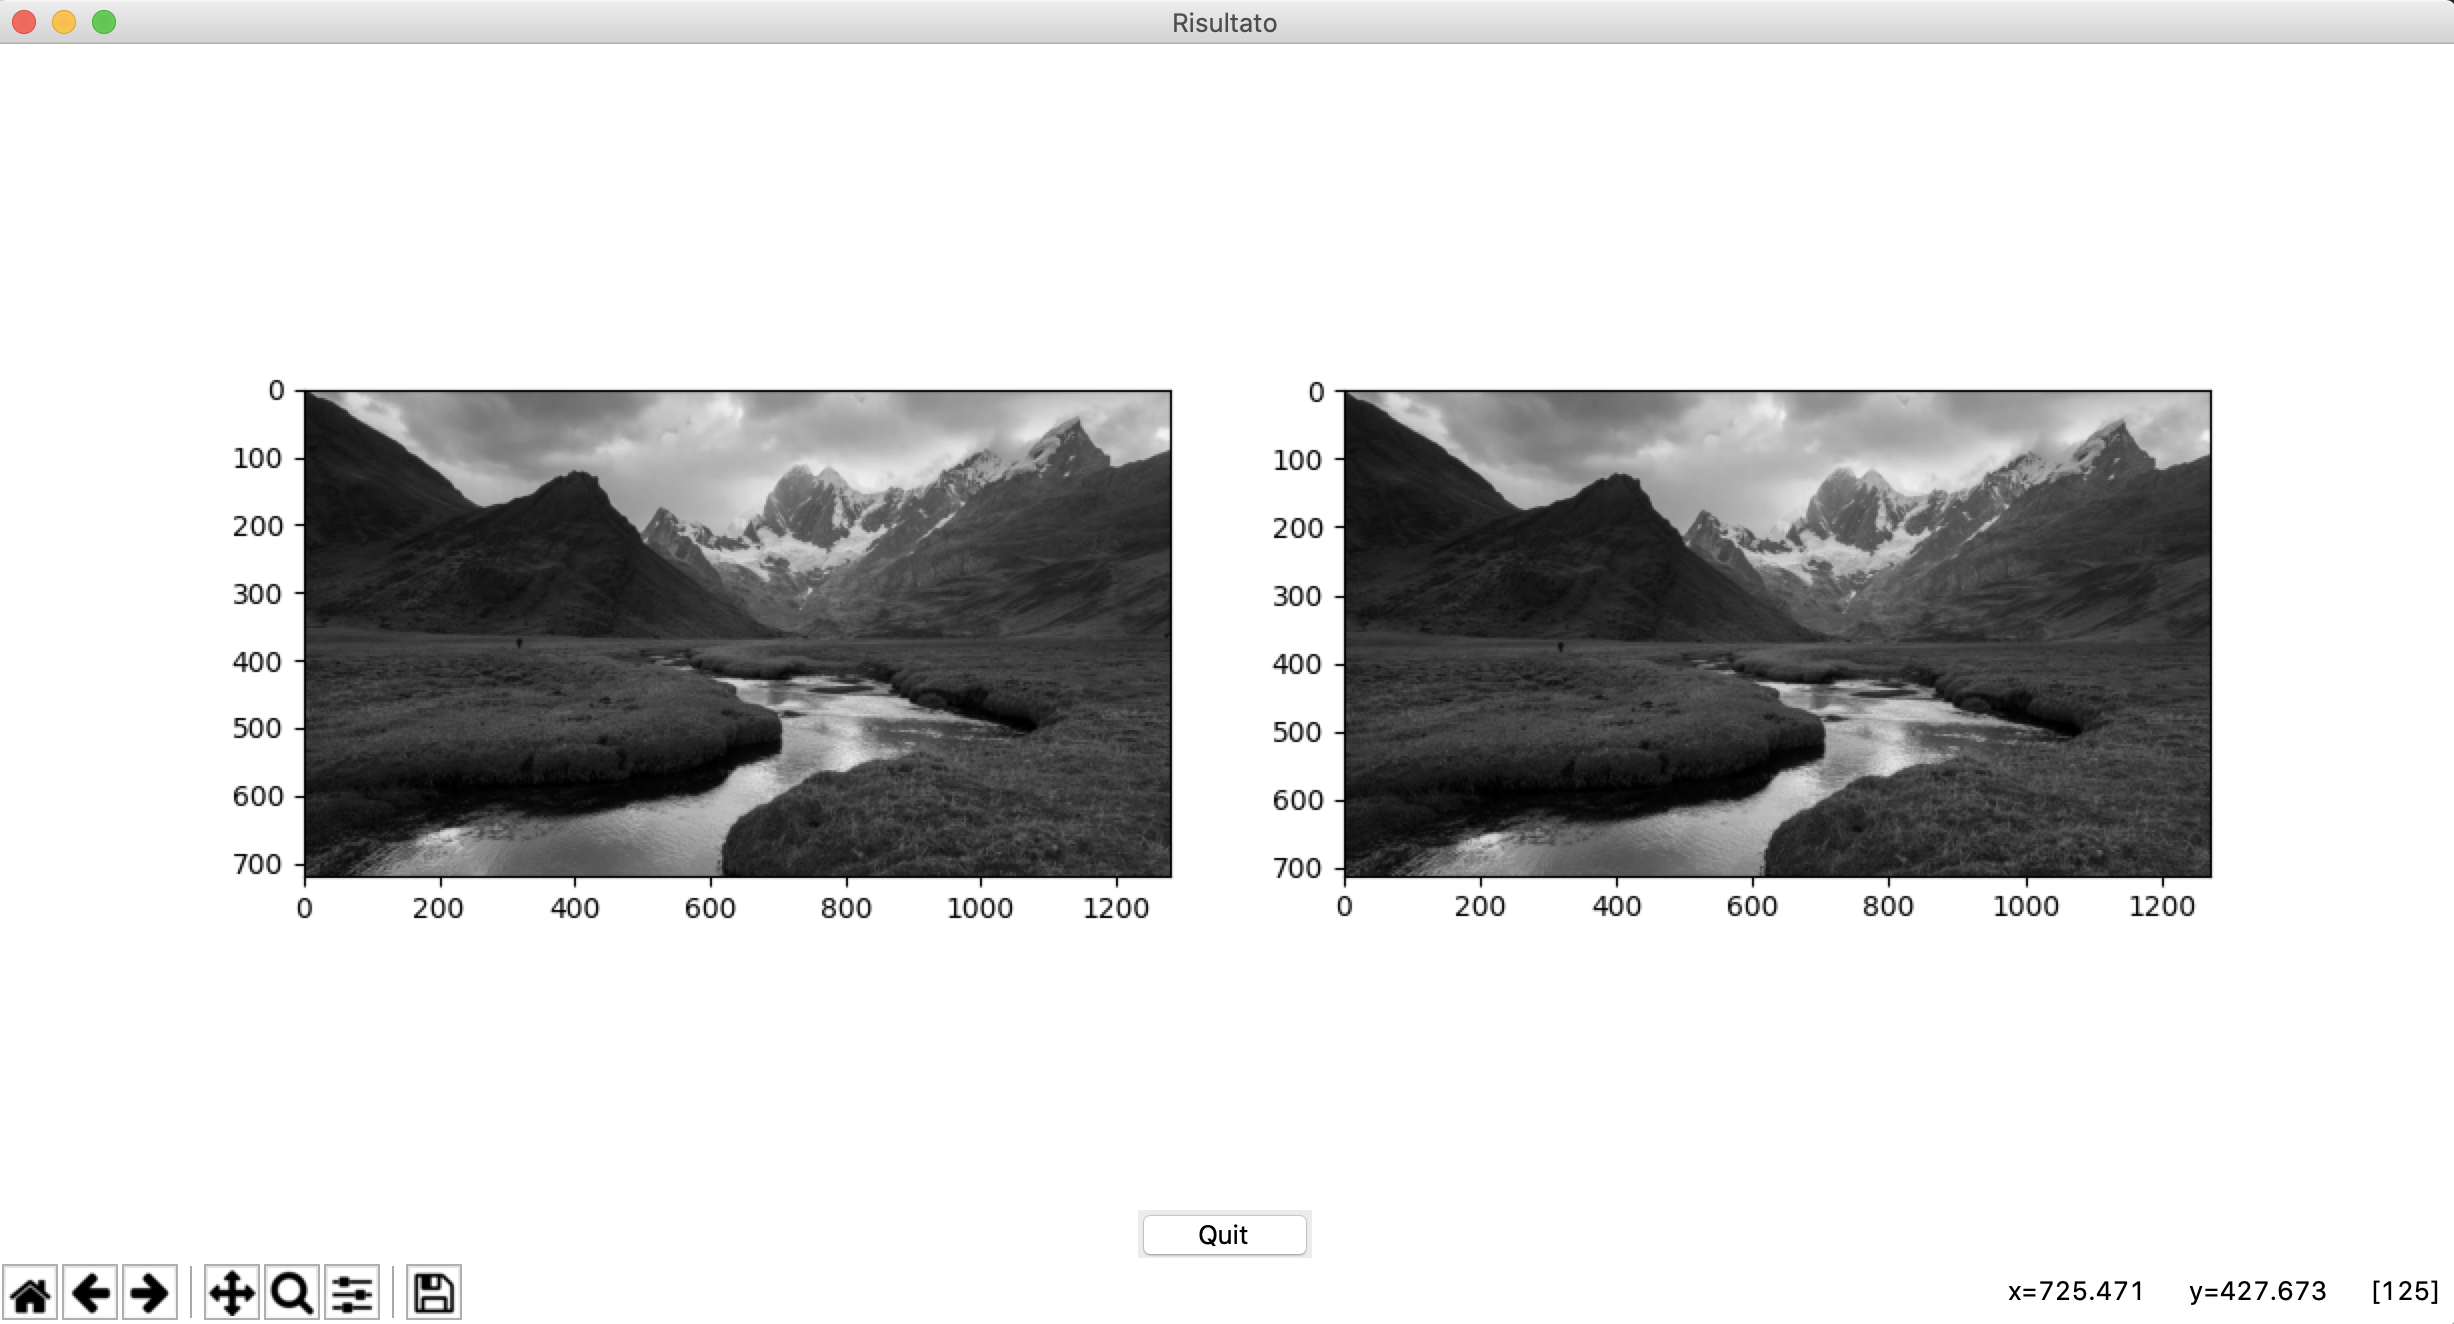
\includegraphics[width=1\linewidth]{risultato}
\end{figure}


\end{document}